% Integration test: compiles every asset handed to the paper inside IEEEtran
% two-column at real column width. Compile: tectonic ieee_snippet_test.tex
% Check the log for Overfull warnings before shipping snippets.
\documentclass[conference]{IEEEtran}
\usepackage{graphicx}
\usepackage{tikz}
\usetikzlibrary{positioning,fit,backgrounds,arrows.meta}
\definecolor{ccblue}{RGB}{33,113,181}
\begin{document}

\title{Snippet Integration Test}
\author{}
\maketitle

\section{Blast-radius figure (for \S VI)}

\begin{figure}[!t]
\centering
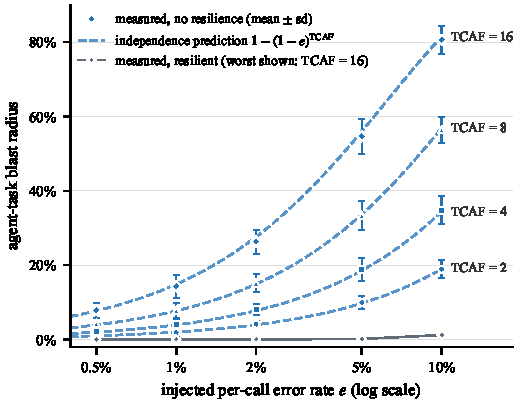
\includegraphics[width=\columnwidth]{fig_blast_radius.pdf}
\caption{Measured agent-task blast radius versus injected per-call error rate
$e$ (log scale), 20 seeds $\times$ 200 tasks per cell (the Table~I sweep).
Without resilience (blue, mean $\pm$ sd) blast radius tracks the independence
prediction $1-(1-e)^{\mathrm{TCAF}}$ (dashed) across the full grid; the \S VII
resilience patterns (gray; worst case, TCAF $=$ 16, shown) recover it to
$\leq$1.2\% everywhere. Generated by \texttt{paper/figures/} in the released
harness.}
\label{fig:blast}
\end{figure}

Body filler to exercise column layout. The tool-call plane compounds per-call
failure into task failure through fan-out; the figure shows the measured sweep
against the closed-form prediction. This paragraph exists only to give the
floats somewhere to sit and to surface overfull boxes at real column width.

\section{Correlated-fault table (for \S VI)}

\begin{table}[!t]
\caption{Measured blast radius (\%) under correlated faults at the same
$\sim$2\% marginal per-call error rate, TCAF $=$ 8 (independence prediction:
14.9\%); mean $\pm$ sd over 50 seeds $\times$ 200 tasks. \emph{Lock-in}: seeds
whose resilient blast radius exceeds 50\% --- a transient fault trips the ETA
breaker, which has no half-open path in the Table~I configuration.
\emph{$+$probes}: same patterns with a breaker probe every 8 skipped calls.}
\label{tab:correlated}
\centering
\scriptsize
\setlength{\tabcolsep}{2.8pt}
\begin{tabular}{lccccc}
\hline
 & marg. & BR, & BR, & lock- & BR,\\
condition & $e$ & no resil. & resilient & in & $+$probes\\
\hline
iid & 2.0\% & 15.1\,$\pm$\,2.6 & 0.0\,$\pm$\,0.1 & 0/50 & 0.0\,$\pm$\,0.1\\
bursts, mean 4 & 2.3\% & 6.0\,$\pm$\,2.2 & 2.1\,$\pm$\,1.0 & 0/50 & 2.1\,$\pm$\,1.0\\
bursts, mean 16 & 2.5\% & 3.5\,$\pm$\,2.7 & 5.3\,$\pm$\,19.5 & 2/50 & 1.6\,$\pm$\,1.9\\
bursts, mean 64 & 2.9\% & 3.2\,$\pm$\,5.0 & 3.0\,$\pm$\,14.1 & 1/50 & 1.4\,$\pm$\,3.3\\
server episodes (20) & 2.4\% & 9.8\,$\pm$\,11.9 & 20.8\,$\pm$\,33.5 & 8/50 & 10.1\,$\pm$\,12.2\\
\hline
\end{tabular}
\end{table}

More filler so the table float has an anchor paragraph and the two-column
balance is realistic. Correlation concentrates failure into heavy tails,
defeats retry budgets, and exposes breaker lock-in.

\section{Reference architecture (for \S VIII)}

\begin{figure}[!t]
\centering
\resizebox{\columnwidth}{!}{% §8 reference-architecture figure body. Drop-in for the paper:
% preamble needs: \usepackage{tikz}
% \usetikzlibrary{positioning,fit,backgrounds,arrows.meta}
% \definecolor{ccblue}{RGB}{33,113,181}
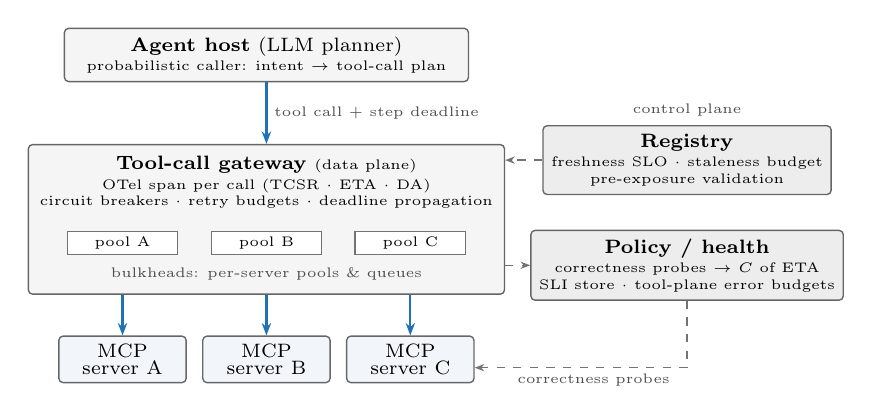
\begin{tikzpicture}[
  font=\scriptsize,
  box/.style={draw=black!60, rounded corners=1.5pt, line width=0.5pt,
              align=center, inner sep=3pt, fill=black!4},
  pool/.style={draw=black!55, line width=0.4pt, inner sep=2pt, fill=white,
               font=\tiny, minimum width=40pt},
  srv/.style={box, fill=ccblue!6},
  ctl/.style={box, fill=black!7, minimum width=78pt},
  dp/.style={-{Stealth[length=4.5pt]}, line width=0.8pt, draw=ccblue},
  cp/.style={-{Stealth[length=3.5pt]}, line width=0.5pt, draw=black!55, dashed},
  lbl/.style={font=\tiny, text=black!70, align=center, inner sep=1pt},
]
% ---- data plane (left column) ----
\node[box, minimum width=146pt] (host) at (0pt, 0pt)
  {\textbf{Agent host} (LLM planner)\\[-1pt]
   {\tiny probabilistic caller: intent $\rightarrow$ tool-call plan}};

\node[align=center, inner sep=0pt] (gwtext) at (0pt, -46pt)
  {\textbf{Tool-call gateway} {\tiny (data plane)}\\[-1pt]
   {\tiny OTel span per call (TCSR $\cdot$ ETA $\cdot$ DA)}\\[-2pt]
   {\tiny circuit breakers $\cdot$ retry budgets $\cdot$ deadline propagation}};
\node[pool] (pa) at (-52pt, -68pt) {pool A};
\node[pool] (pb) at (0pt, -68pt) {pool B};
\node[pool] (pc) at (52pt, -68pt) {pool C};
\node[lbl] (bh) at (0pt, -79pt) {bulkheads: per-server pools \& queues};
\begin{scope}[on background layer]
  \node[box, fit=(gwtext)(pa)(pc)(bh), inner sep=4pt] (gw) {};
\end{scope}

\node[srv, minimum width=46pt] (sa) at (-52pt, -110pt) {MCP\\[-2pt] server A};
\node[srv, minimum width=46pt] (sb) at (0pt, -110pt)   {MCP\\[-2pt] server B};
\node[srv, minimum width=46pt] (sc) at (52pt, -110pt)  {MCP\\[-2pt] server C};

\draw[dp] (host) -- node[lbl, right=1.5pt] {tool call + step deadline} (gw);
\draw[dp] ([xshift=-52pt]gw.south) -- (sa.north);
\draw[dp] (gw.south) -- (sb.north);
\draw[dp] ([xshift=52pt]gw.south) -- (sc.north);

% ---- control plane (right column) ----
\node[ctl] (reg) at (152pt, -38pt)
  {\textbf{Registry}\\[-1pt]
   {\tiny freshness SLO $\cdot$ staleness budget}\\[-2pt]
   {\tiny pre-exposure validation}};
\node[ctl] (pol) at (152pt, -76pt)
  {\textbf{Policy / health}\\[-1pt]
   {\tiny correctness probes $\rightarrow$ $C$ of ETA}\\[-2pt]
   {\tiny SLI store $\cdot$ tool-plane error budgets}};
\node[lbl] at (152pt, -20pt) {control plane};

\draw[cp] (reg.west) -- (reg.west -| gw.east);
\draw[cp] (pol.west -| gw.east) -- (pol.west);
\draw[cp] (pol.south) |- node[lbl, below=1pt, pos=0.72] {correctness probes}
  ([yshift=-3pt]sc.east);
\end{tikzpicture}
}
\caption{The managed tool-call plane (\S VIII). Solid blue --- data plane:
every call crosses a gateway that emits an OpenTelemetry span carrying
TCSR/ETA/DA attributes, enforces circuit breakers and retry budgets,
propagates deadlines, and isolates servers behind per-server bulkhead pools.
Dashed gray --- control plane: a registry with a freshness SLO performs
pre-exposure validation and feeds the gateway its validated tool set; a
policy/health layer ingests the gateway's spans/SLIs and runs correctness
probes (the $C$ factor of ETA) against servers. Deliberately analogous to a
service-mesh data plane plus control plane.}
\label{fig:arch}
\end{figure}

Final filler paragraph. The architecture is the operational complement of the
SLIs: the gateway is where TCSR, ETA, and DA are emitted and enforced, and the
control plane is where tool-plane error budgets are spent.

\end{document}
